\documentclass[a4paper,12pt]{report}

% Page layout
\usepackage[left=2.5cm,right=2.5cm,top=2.5cm,bottom=2.5cm]{geometry}

% Figures
\usepackage[margin=\the\parindent,small,bf,sf]{caption}
\usepackage{
}
\usepackage{pdfpages}
\setlength{\abovecaptionskip}{7.5pt}  % spacing above and below captions
\newcommand*{\WaterMark}[2][0.2\paperwidth]{\AddToShipoutPicture*{\AtTextCenter{\parbox[c]{0pt}{\makebox[0pt][c]{\includegraphics[width=#1]{#2}}}}}}

% Font and text
\usepackage[english]{babel}
\usepackage{microtype}
\usepackage{setspace}
\usepackage{lmodern}
\newcommand{\myemph}[1]{{\sffamily\bfseries#1}}
\sloppy
\onehalfspacing

% Headings
\usepackage[raggedright,sf,bf]{titlesec}
\titlelabel{\thetitle.\ }
\titleformat{\chapter}[display]{\huge\bfseries\sffamily}{\chaptertitlename\ \thechapter}{15pt}{\Huge \raggedright}
% \titleformat{\chapter}[display]{\centering\huge\bfseries\sffamily}{\chaptertitlename\ \thechapter:}{15pt}{}
\titlespacing*{\chapter}{0pt}{0pt}{40pt}  % remove spacing before chapter headings

% Table of contents
\makeatletter
\let\originall@chapter\l@chapter
\def\l@chapter#1#2{\originall@chapter{{\sffamily #1}}{#2}}
\makeatother
\let \savenumberline \numberline
\def \numberline#1{\savenumberline{#1.}}

% Mathematics
\usepackage[cmex10]{amsmath}
\usepackage{amssymb}
\usepackage{cancel}
\DeclareMathOperator*{\argmax}{arg\,max}
\newcommand{\T}{^\textrm{T}}
\newcommand{\tr}{\textrm{tr}}
\renewcommand{\vec}[1]{\boldsymbol{\mathbf{#1}}}
\newcommand{\defeq}{\triangleq}

% Tables
\usepackage{booktabs}
\usepackage{tabularx}
\usepackage{multirow}
\newcommand{\mytable}{
    \centering
    \small
    \renewcommand{\arraystretch}{1.2}
    }
\renewcommand{\tabularxcolumn}[1]{m{#1}}
\newcolumntype{C}{>{\centering\arraybackslash}X}
\newcolumntype{L}{>{\raggedright\arraybackslash}X}

% Header and footer
\usepackage{fancyhdr}
\pagestyle{fancy}
\fancyhf{}
\renewcommand{\sectionmark}[1]{\markright{\normalsize \thesection.\ #1}}
\fancyhead[C]{\nouppercase{\textit{\rightmark}}}
\fancyhead[RO]{\thepage}
% \fancyhead[LE]{\thepage}  % double-sided printing
\fancyfoot{}
\setlength\headheight{14.5pt}
\renewcommand{\headrulewidth}{0pt}
\fancypagestyle{plain}{\fancyhead{}
                       \renewcommand{\headrulewidth}{0pt}
                       \fancyfoot[C]{\thepage}}

% Pseudo-code
\usepackage{algorithm}  % should go before \usepackage{hyperref}

% Table of contents and hyperlinks
\usepackage{hyperref}
\hypersetup{colorlinks=true,linktoc=all,citecolor=black,linkcolor=black}
\usepackage[nottoc]{tocbibind}

% Pseudo-code
\usepackage{algpseudocode}  % should go after \usepackage{hyperref}
\renewcommand{\thealgorithm}{\arabic{chapter}.\arabic{algorithm}} 
%\captionsetup[algorithm]{labelfont={bf,sf},font=small,labelsep=colon}

% Bibliography
\usepackage{cite}  % automatically reorder inline citations
\bibliographystyle{IEEEtran}

\usepackage{caption}
\usepackage{subcaption}

% Fix titlesec issue
\usepackage{etoolbox}
\makeatletter
\patchcmd{\ttlh@hang}{\parindent\z@}{\parindent\z@\leavevmode}{}{}
\patchcmd{\ttlh@hang}{\noindent}{}{}{}
\makeatother


\begin{document}

% Front matter
\graphicspath{{frontmatter/fig/}}
\pagenumbering{Alph}

\begin{titlepage}
\begin{center}


\includegraphics[width=10cm]{USlogo-top}

\vfill

{\sffamily \bfseries \huge A critical analysis of major design flaws in the Death Star \par}

\vfill

{\large {\Large Obi-Wan Kenobi} \\ 99652154 \par}

\vfill

\vfill

{Report submitted in partial fulfilment of the requirements of the module \\
Project (E) 448 for the degree Baccalaureus in Engineering in the Department of
Electrical and Electronic Engineering at Stellenbosch University. \par}

\vfill

{\large {Supervisor}: Dr L. Skywalker} %\\
% Department of Electrical and Electronic Engineering \par}

\vfill

{\Large October 2099}
\end{center}
\end{titlepage}

%\graphicspath{{frontmatter/fig/}}
\pagenumbering{Alph}

\begin{titlepage}
\begin{center}

%
\includegraphics[width=10cm]{USlogo-top}

\WaterMark{UScrest-WM}

~\vspace{4.5em}

{\sffamily \bfseries \huge A critical analysis of major design flaws in the Death Star \par}

\vspace{7em}

{\large {\Large Obi-Wan Kenobi} \\ 99652154 \par}

\vspace{8em}

{\large Thesis presented in partial fulfilment of the requirements for the degree of \\ Master of Engineering (Electronic) in the Faculty of Engineering at Stellenbosch University. \par}

\vfill

{\large {Supervisor}: Dr H. Kamper \\
Department of Electrical and Electronic Engineering \par}

%\vfill
\vspace{10em}

{\Large October 2099}
\end{center}
\end{titlepage}

\pagenumbering{roman}
\chapter*{Acknowledgements}
% \addcontentsline{toc}{chapter}{Acknowledgements}
\makeatletter\@mkboth{}{Acknowledgements}\makeatother

I would like to thank my dog, Muffin. I also would like to thank the inventor of the incubator; without him/her, I would not be here. Finally, I would like to thank Dr Herman Kamper for this amazing report template.
%\chapter*{Declaration}
\newpage
\pagestyle{plain}
\addcontentsline{toc}{chapter}{Declaration}
\makeatletter\@mkboth{}{Declaration}\makeatother

\centerline{
\includegraphics[width=8cm]{USlogo-top}}
\vspace*{-10pt}

\section*{\centering Plagiaatverklaring / \textit{Plagiarism Declaration}}

\vspace*{5pt}

\begin{enumerate}
    \item Plagiaat is die oorneem en gebruik van die idees, materiaal en ander intellektuele eiendom van ander persone asof dit jou eie werk is.\\
    \textit{Plagiarism is the use of ideas, material and other intellectual property of another's work
        and to present is as my own.}
    
    \item Ek erken dat die pleeg van plagiaat 'n strafbare oortreding is aangesien dit 'n vorm van diefstal is.\\
    \textit{I agree that plagiarism is a punishable offence because it constitutes theft.}
    
    \item Ek verstaan ook dat direkte vertalings plagiaat is. \\
    \textit{I also understand that direct translations are plagiarism.}
    
    \item Dienooreenkomstig is alle aanhalings en bydraes vanuit enige bron (ingesluit die internet) volledig verwys (erken). Ek erken dat die woordelikse aanhaal van teks sonder aanhalingstekens (selfs al word die bron volledig erken) plagiaat is. \\
    \textit{Accordingly all quotations and contributions from any source whatsoever (including the internet) have been cited fully. I understand that the reproduction of text without quotation marks (even when the source is cited) is plagiarism}
    
    \item Ek verklaar dat die werk in hierdie skryfstuk vervat, behalwe waar anders aangedui, my eie oorspronklike werk is en dat ek dit nie vantevore in die geheel of gedeeltelik ingehandig het vir bepunting in hierdie module/werkstuk of 'n ander module/werkstuk~nie. \\
    \textit{I declare that the work contained in this assignment, except where otherwise stated, is my original work and that I have not previously (in its entirety or in part) submitted it for grading in this module/assignment or another module/assignment.}
\end{enumerate}

\vfill

\noindent \begin{tabularx}{1.0\linewidth}{|L|L|}
    \hline
    \vspace{1cm} {Studentenommer / \textit{Student number}} & \vspace{1cm} {Handtekening / \textit{Signature}} \\
    \hline
    \vspace{1cm} {Voorletters en van / \textit{Initials and surname}} & \vspace{1cm} {Datum / \textit{Date}} \\
    \hline
\end{tabularx}

\vspace{15pt}

% The old declaration

%I, the undersigned, hereby declare that the work contained in this report is my own original work unless otherwise stated.
%
%% Afrikaans:
%% Hiermee verklaar ek, die ondergetekende, dat die werk in hierdie verslag vervat my eie oorspronklike werk is, tensy anders vermeld.
%
%\vspace{2.5cm}
%
%\begin{table}[h]
%\begin{tabular}{@{}p{2.5cm}p{5cm}}
%    Signature: & \dotfill \\
%    & \multicolumn{1}{c}{Obi-Wan Kenobi} \\
%    ~\vspace{1cm} \\
%    Date: & \dotfill \\
%\end{tabular}
%\end{table}
%
%\vfill
%
%\begin{center}
%    Copyright \textcopyright\ 2099 Stellenbosch University \\
%    All rights reserved
%\end{center}


\chapter*{Abstract}
\addcontentsline{toc}{chapter}{Abstract}
\makeatletter\@mkboth{}{Abstract}\makeatother

\subsubsection*{English}

The English abstract.

\selectlanguage{english}
\tableofcontents
\listoffigures
\listoftables
\chapter*{Nomenclature\markboth{}{Nomenclature}}
\addcontentsline{toc}{chapter}{Nomenclature}

% \vspace*{-3mm}
\subsubsection*{Variables and functions}

\begingroup
\renewcommand{\arraystretch}{1.2}
\renewcommand{\tabularxcolumn}[1]{p{#1}}
\begin{tabularx}{\textwidth}{@{}p{2.5cm}L}
    $p(x)$ & Probability density function with respect to variable $x$.\\
\end{tabularx}
\endgroup

\subsubsection*{Acronyms and abbreviations}

\begingroup
\renewcommand{\arraystretch}{1.2}
\begin{tabular}{@{}p{2.5cm} l}
    RL		& Reinforcement Learning \\
    SARSA	& State-Action-Reward-State=Action \\
    Q-learning	& Q value learning \\
    MDP		& Markov Decision
    Process \\
\end{tabular}
\endgroup

\newpage
\pagenumbering{arabic}

% Contents
\graphicspath{{introduction/fig/}}

\chapter{Introduction}
\label{chap:introduction}

\section{Problem Statement and Project Objective}
In robotics, a manipulator (ie. a robotic arm) is a device used to manipulate objects in its environment. When the manipulation task is relatively complex, it is often difficult or even impossible for a human to direct how the robot should act. One possible solution is that the robot learn by itself which actions are best, which can be done through reinforcement learning. A popular method for doing developing reinforcement learning algorithms for robotics is to first solve similar, less complex problems.

In this project reinforcement learning is used to solve sliding puzzle. An example of a sliding puzzle being solved can be seen in Figure \ref{fig:sliding_puzzle_figs}. The objective of this project is to solve a shuffled puzzle with the minimum amount of moves using reinforcement learning. The rules of the game are explained in the next section. 

\section{Background}

The sliding puzzle is a game with a history dating back to the 1870's \cite{15_puz}. The game consists of $N^{2}-1$ tiles arranged on an NxN grid with one empty tile. The tiles are numbered 1 to N. A possible configuration of a 3x3 puzzle is shown in Figure \ref{fig:sfig1}. The puzzles state can be changed by sliding one of the numbered tiles, next to the empty tile, into the place of the empty tile. The empty tile then takes the place of the numbered tile. This can visually be seen between Figures \ref{fig:sfig1}
and \ref{fig:sfig2} where tile number 6 moves right in the transition between Figures \ref{fig:sfig1}
and \ref{fig:sfig2}. We will denote the action that can occur in a certain state by the possible movements the empty tile can move. Which will be defined as $A_s = {up, down, left, right}$.

The sliding puzzle is a game with a history dating back to the 1870's \cite{15_puz}. Many solutions have been thought up to solve such puzzles, which include using search algorithms\cite{search_alg}. The rules of the game are that the only tiles that can move are the ones next to the tile with no number, known as the 'blank tile'. Additionally only one tile can be moved at a time. The final puzzle configuration is shown in \ref{fig:sfig4}, where all the tiles are placed in ascending order read left to right and top to bottom. The aim of the game is to arrange a shuffled puzzle into the final puzzle configuration by moving one tile at a time.

\begin{figure}[!htb]
	\centering
	\begin{subfigure}{.4\textwidth}
		\centering
		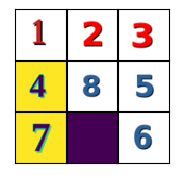
\includegraphics[width=.8\linewidth]{game_states/31.png}
		\caption{Puzzle with tiles 5,6,8 and blank in the incorrect positions}
		\label{fig:sfig1}
	\end{subfigure}%
	\begin{subfigure}{.4\textwidth}
		\centering
		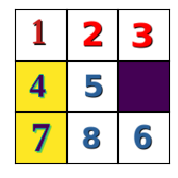
\includegraphics[width=.8\linewidth]{game_states/32.png}
		\caption{Puzzle with tiles 5,8 and blank in the incorrect positions}
		\label{fig:sfig2}
	\end{subfigure}
	\begin{subfigure}{.4\textwidth}
		\centering
		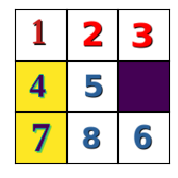
\includegraphics[width=.8\linewidth]{game_states/33.png}
		\caption{Puzzle with tiles 8 and blank in the incorrect positions}
		\label{fig:sfig3}
	\end{subfigure}
	\begin{subfigure}{.4\textwidth}
		\centering
		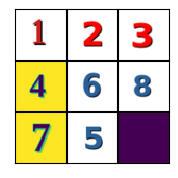
\includegraphics[width=.8\linewidth]{game_states/34.png}
		\caption{Solved puzzle}
		\label{fig:sfig4}
	\end{subfigure}
	\caption{Figures of a 3x3 sliding puzzle being solved}
	\label{fig:sliding_puzzle_figs}
\end{figure}

\section{Document Outline} 
In Chapter \ref{chap:Literature_Review} we will look at a paper which used an alternate approach to solve a 16 tile sliding puzzle.
Chapter \ref{chap:MDP} describes in detail theory relating to Markov decision processes.
Chapter \ref{chap:RL} discusses in detail the dynamic programming and reinforcement learning techniques which will be used to solve our puzzle problem.

In Chapter \ref{chap:System_Design} the theory of reinforcement learning is applied to solve sliding puzzles. In the same chapter we 

{\color{red}Rather how you used the theory of RL to design the solution to the sliding puzzle problem. Do this mathematically. Talk about things like the size of the state space, the sequential agents that you trained, how you decided on algorithms or hyperparameters.}

Chapter \ref{chap:Experiments_and_Results} contains tests and verification that our solution works using the results of various experiments.
Chapter \ref{chap:conclusion} concludes the report.
\graphicspath{{Literature\_Review/fig}}
\chapter{Literature Review/Study/Related work}
\label{chap:Literature_Review}

\section{Introduction}
Reinforcement learning is a method of learning what to do by linking states to actions with a numerical reward incurred for every state-action pair. The final goal of RL is to find a path of states and actions with the maximum amount of reward. \cite{sutton_barto} This path is typically described as a policy $\pi$.

\section{Solving sliding puzzle using value iteration}
In this section a few terms will be used which are fully described in the theory chapters \ref{chap:MDP} and \ref{chap:RL}. These terms include value iteration and policy iteration.

A 4x4 puzzle solution is investigated in \cite{15-puzzle_value_iteration}.
The method they use is a variation of value iteration. The amount of states in a 4x4 puzzle is approximately 10\^13 elements.
It was found in \cite{15-puzzle_value_iteration} that value iteration is indeed a feasible approach if the value iteration algorithm is altered so that the only a subset of the entire state space is used sequentially until a solution is found. 

This reducing of the state space is similar to what will later be done in this report. However the method we use to reduce the state space is by having our algorithm be guided somewhat by how a human would solve a puzzle, by doing the edges first. Additionally that we use a different reinforcement learning method known as policy iteration.


Solutions to sliding puzzles can also been found by using search algorithms such as A* and IDA*
\cite{search_alg}.

\graphicspath{{MDP/fig/}}

\chapter{Markov Decision Processes}
\label{chap:MDP}
\section{Introduction}

In order to describe reinforcement learning techniques, we first have to have a way of mathematically defining reinforcement learning problems. In this chapter, we do so by formally introduce the concept of Markov decision processes (MDPs). This chapter introduces the key concepts required to address the reinforcement learning problem. These concepts includes, state and action space, returns, value functions and Bellman equations.
The majority of the theory discussed in this chapter is based on the work by Sutton and Barto \cite{sutton_barto}.
\section{Definition of a MDP}
A Markov decision process is a stochastic, discrete, time controlled process. What this means is that a MDP is a partially controlled and partially random process \cite{sutton_barto}.
In general RL problems can be described using MDPs \cite{David_Silver}. 
Paul Weng states that, MDP's are described by the following: state-space S, action-space A, state transition probability $P^{a}_{ss'}$, reward function $R^{a}_{s}$ and discount factor $\gamma$\cite{MDP_Paul_Weng}. These variables can be denoted in a 5-tuple as
\begin{equation}
	(S,A,P^{a}_{ss'},R^{a}_{s},\gamma)
\end{equation}
 where,
\begin{itemize}
	\item S is a finite set of states with state s $\in$ S
	\item A is a finite set of actions with action a $\in$ A
	\item $P^{a}_{ss'}$ is a matrix of probabilities which predicts the next state s', where\\ $P^{a}_{ss'} = P(S_{t+1} = s' | S_t = s,A_t = a) $
	\item $R^{a}_{s}$ is the immediate reward after transitioning from state s to s' using action a, where $R^{a}_{s} = E[R_{t+1}|S_t =s, A_t =a]$
	\item $\gamma$ $\in$ [0,1] is the discount factor applied to the reward
\end{itemize}
In an MDP, the assumption is that all the states have the Markov property \cite{sutton_barto}. This means that
\begin{equation}
	P[S_{t+1}|S_{t}] = P[S_{t+1}|S_{1},...,S_{t}].
\end{equation}
In other words, the probability of transitioning to state $S_{t+1}$ given state $S_t$, must be equal to the probability of transitioning to state $S_{t+1}$ given all states $S_1$ to $S_t$. This means that the current state is required to contain all the information of the previous states.

\section{Value function and policies}
The return $G_t$ is the total sum of the reward at each time step, multiplied by a constant diminishing factor $\gamma$.
The discount $\gamma$ $\in$ [0,1] determines the present value of future reward $R_{t}$.

\begin{align}
	G_t &= R_{t+1}+\gamma R_{t+2} +\gamma^2 R_{t+3}+ ... \nonumber\\
	&= \sum_{k=0}^{\infty}\gamma^{k} R_{t+k+1}
	\label{eq:G_t}
\end{align}

For $\gamma=0$, the return $G_t$ only depends on the single reward that can be obtained in the next step, namely $R_{t+1}$. When $\gamma=0$ the return $G_t$ is 'short-sighted'. For $\gamma=1$ on the other hand, the return depends on all the rewards that are projected to be obtained until the process terminates. $G_t$ is thus "far-sighted" for $\gamma=1$ \cite{sutton_barto}.
What can also note is that using a discount factor between 0 and 1 makes the return finite because $R_{t+k+1}$ is finite and
\begin{equation}
	\sum_{k=0}^{\infty}\gamma^{k}=\frac{1}{1-\gamma}\hspace{5pt},
\end{equation}
which is finite for $\gamma$ $\in$ [0,1]. \\
The probability that the agent will choose a specific action given the state is called its policy $\pi(a|s)$. Mathematically this is defined as
\begin{equation}
	\pi(a|s) = P[A_t = a, S_t = s].
\end{equation}
Another important definition is the value function v(s) defined as
\begin{equation}
	v(s) = E[G_t | S_t = s].
\end{equation}
This equation shows that the value function v(s) is the expected return given that v(s) is evaluated in state s at time-step t.
\section{Bellman Expectation Equation}
Sutton and Barto \cite{sutton_barto} further decomposes v(s) so that it becomes a recursive function as follows
\begin{align}
	v(s) &= E[G_t | S_t = s]\\
	&= E[R_{t+1} + \gamma R_{t+2} + \gamma^{2} R_{t+3} + ...|S_t = s]\\
	&= E[R_{t+1} + \gamma (R_{t+2} + \gamma R_{t+3} + ...)|S_t = s]\\
	&= E[R_{t+1} + \gamma G_{t+1}|S_t = s]\\
	&= E[R_{t+1} + \gamma v(S_{t+1})|S_t = s].
	\label{bellmanv1}
\end{align}
This means that v(s) only depends on $R_{t+1}$ (the reward that can be obtained in the next step) and $\gamma v(S_{t+1})$, the discounted value function at time t+1.
What has been defined in equation \ref{bellmanv1} is known as the Bellman equation.\cite{sutton_barto}
Sutton and Barto then defines the value function given that the agent follows the policy $\pi$ as
\begin{equation}
	v_{\pi}(s) = E_{\pi}[G_t | S_t = s].
\end{equation}
Additionally, they define the action-value function (q-function),
\begin{equation}
	q_{\pi}(s,a) = E_{\pi}[G_t | S_t = s,A_t = a].
\end{equation}
The q-function is defined as the expected return of taking action a from state s and thereafter following policy $\pi$. What can be noted is that v(s) is a prediction of what the value for being in a certain state is, which is related to planning. While q(s,a) is the value for being in a certain state and taking an action, which relates to control. 

Once again, Sutton and Barto \cite{sutton_barto} decomposes the state-value and action-value functions to be in the form of the Bellman Equation in equation \ref{bellmanv1}. This results in the Bellman \textit{expectation} equations
\begin{align}
	v_{\pi}(s)	&= E_{\pi}[R_{t+1} + \gamma v_{\pi}(S_{t+1})|S_t = s]\\
	&= \sum_{a'\in A}\pi(a|s)(R^{a}_s+\gamma\sum_{s'\in S}P^{a}_{ss'}v_\pi(s'))
	\label{bellmanv2}
\end{align}
and
\begin{align}
	q_{\pi}(s,a)	&= E_{\pi}[R_{t+1} + \gamma q_{\pi}(S_{t+1},A_{t+1})|S_t = s,A_t = a]\\
	&= R^{a}_s +\gamma \sum_{s'\in S}P^{a}_{ss'}\sum_{a'\in A}\pi(a'|s')q_\pi(s',a').
	\label{bellmanq}
\end{align}
Equation \ref{bellmanv2} can be placed into vector form as:
\begin{equation}
	v_\pi = R^{\pi} + \gamma P^{\pi}v_\pi
\end{equation}
Which has the solution:
\begin{equation}
	v_\pi = (I - \gamma P^{\pi})^{-1}R^{\pi}
	\label{bellman_matrix_form}
\end{equation}
Equation \ref{bellman_matrix_form} is a concise formula which is easily implemented in code, with an example implementation shown in {\color{red} \huge{INSERT GRID WORLD EXAMPLE HEREE}}

\section{Optimal Policies and Bellman Optimality Equations}
Sutton and Barto now defines what is known as the optimal policy, which is essentially a set of state and action pairs which leads to the maximum value of $q_\pi(s,a)$ as:
\begin{align}
	\pi_{*}(a|s)=\begin{cases}
		1, & \text{if a = $\argmax\limits_{a \in A}q_* (s,a)$}\\
		0, & \text{otherwise}
	\end{cases}
	\label{eq:pi_*}
\end{align}
There always exists an optimal deterministic policy for any MDP \cite{sutton_barto}. We only need to know $q_* (s,a)$ to know the optimal policy. This is important because the optimal policy describes which actions must be taken to maximize rewards, which is precisely the goal of RL.
Sutton and Barto \cite{sutton_barto} then defines what is know as the Bellman \textit{optimality} equations.
\begin{equation}
	v_*(s) = \max\limits_{a}(R^{a}_s+\gamma\sum_{s'\in S}P^{a}_{ss'}v_*(s'))
	\label{bellmanv*}
\end{equation}
and
\begin{equation}
	q_*(s,a) = R^{a}_s +\gamma \sum_{s'\in S}P^{a}_{ss'}\max\limits_{a'}q_*(s',a').
	\label{bellmanq*}
\end{equation}
What equation \ref{bellmanv*} represents is the maximum return that can be obtained from state s, when following the optimal policy $\pi_*$. Equation \ref{bellmanq*} represents the maximum return that can be obtained by taking action a state s and thereafter following the policy.
At this point, we have outlined a mathematical background for reinforcement learning problems.
In the next two chapters we will discuss methods of solving the MDP and obtaining the optimal state-value and action-value functions. 


\graphicspath{{RL/fig}}
\chapter{Dynamic Programming and Reinforcement Learning}
\label{chap:RL}

\section{Introduction}
This chapter can be divided into three sections. Dynamic programming which \textbf{solves} a \textit{\textbf{known}} MDP, model-free prediction which \textbf{estimates} an \textit{\textbf{unknown}} MDP and model-free control which \textbf{optimizes} the value function of an \textit{\textbf{unknown}} MDP.

\section{Dynamic Programming}
\subsection{Background}
Dynamic programming is a method to solve problems by using a divide and conquer approach. That is to say a problem is broken into smaller sub-problems and then solved.
There are two properties that must be met for a problem to be solvable via Dynamic Programming: Optimal substructure and Overlapping sub-problems. \cite{David_Silver}
\begin{itemize}
	\item Optimal substructure requires that the solution be able to be decomposed into sub-problems.
	\item Overlapping sub-problems requires that the sub-problems occur many times over, meaning that the solution can be cached and reused.
\end{itemize}

Markov decision processes satisfies both of these conditions. The Bellman equation provides a recursive decomposition which fulfills the Optimal substructure property. While the value function caches and reuses solutions satisfying the Overlapping sub-problems condition. \cite{David_Silver}\\

\subsection{Iterative Policy Evaluation}
In order to evaluate the value that a certain policy has, we use a method called \textit{Iterative Policy Evaluation}. Figure \ref{fig:iterative_policy_evaluation} shows the mathematics which describes Iterative Policy Evaluation in both summation and vector form. What the diagram  at the top of Figure \ref{fig:iterative_policy_evaluation} represents is the value function being calculated for an action 'a' to an intermediary state represented by the black dot. The environments reaction is then also accounted for from the intermediary state to state s' resulting in reward r. The environments information is contained in the transition probability matrix $P^\pi$.

We then use state s' as the new start state s and repeat the same calculation.
The value function is updated continuously until the difference between $v^{k}$ and $v^{k+1}$ is determined negligible.

\begin{figure}
	\centering
	\begin{subfigure}{.49\textwidth}
		\centering
		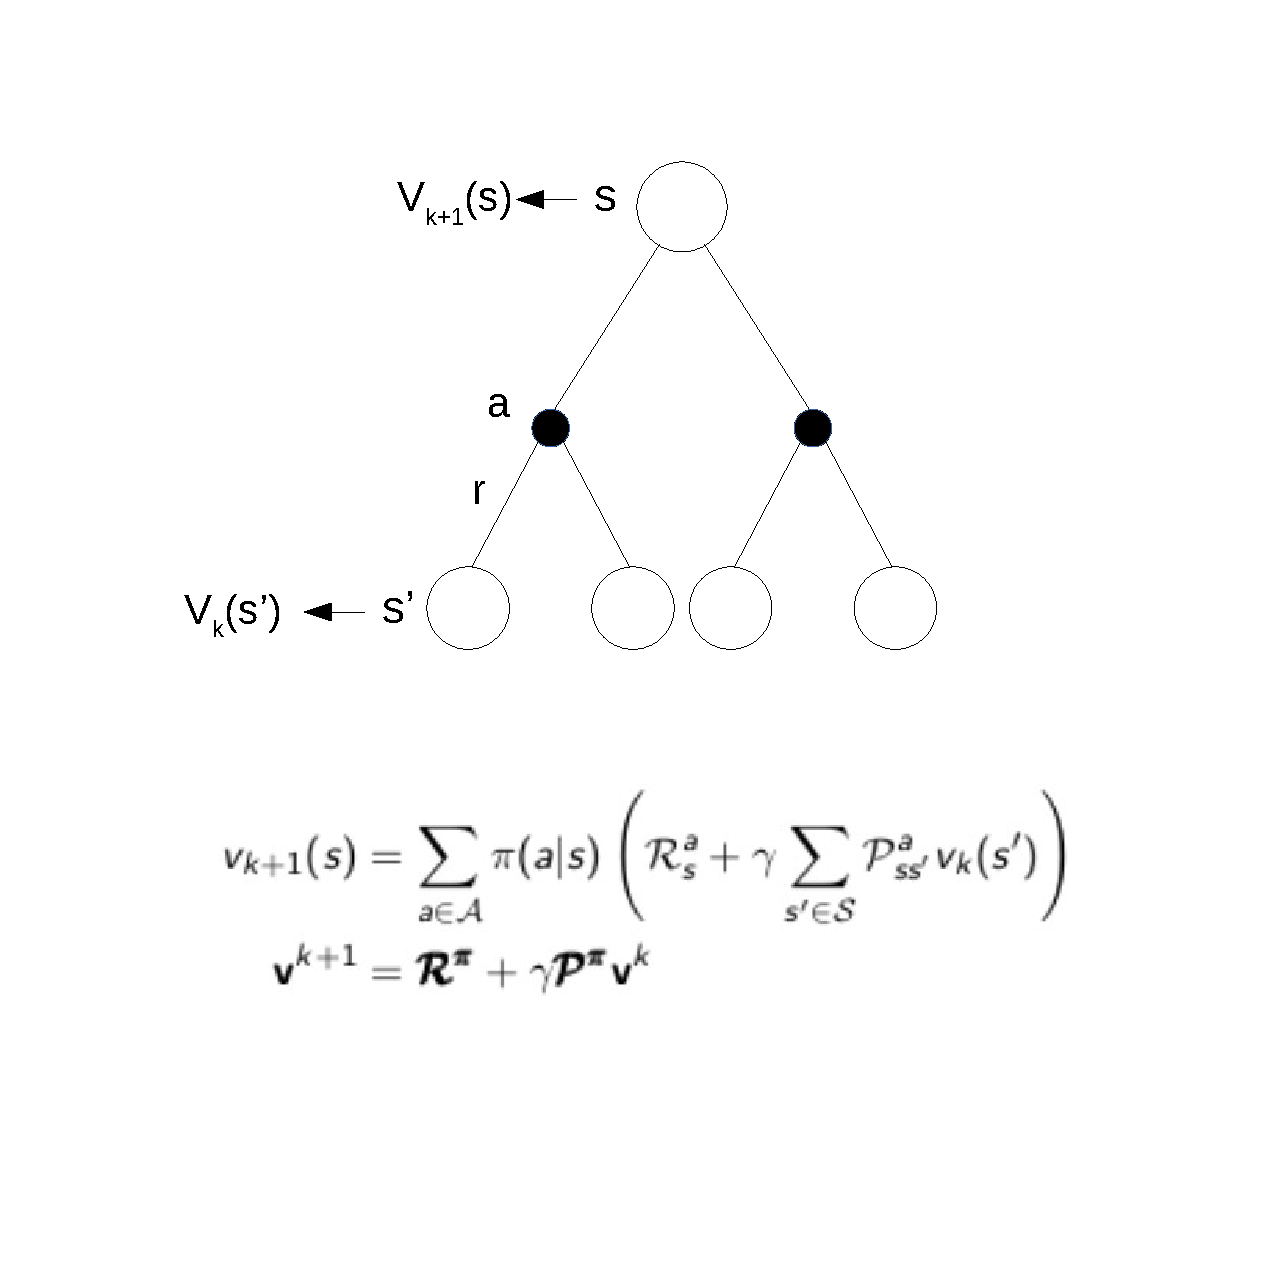
\includegraphics[width=1\linewidth]{MDP/fig/Iterative_Policy_Evaluation.png}
		\caption{Iterative policy Evaluation\cite{David_Silver}}
		\label{fig:iterative_policy_evaluation}
	\end{subfigure}
	\begin{subfigure}{.49\textwidth}
		\centering
		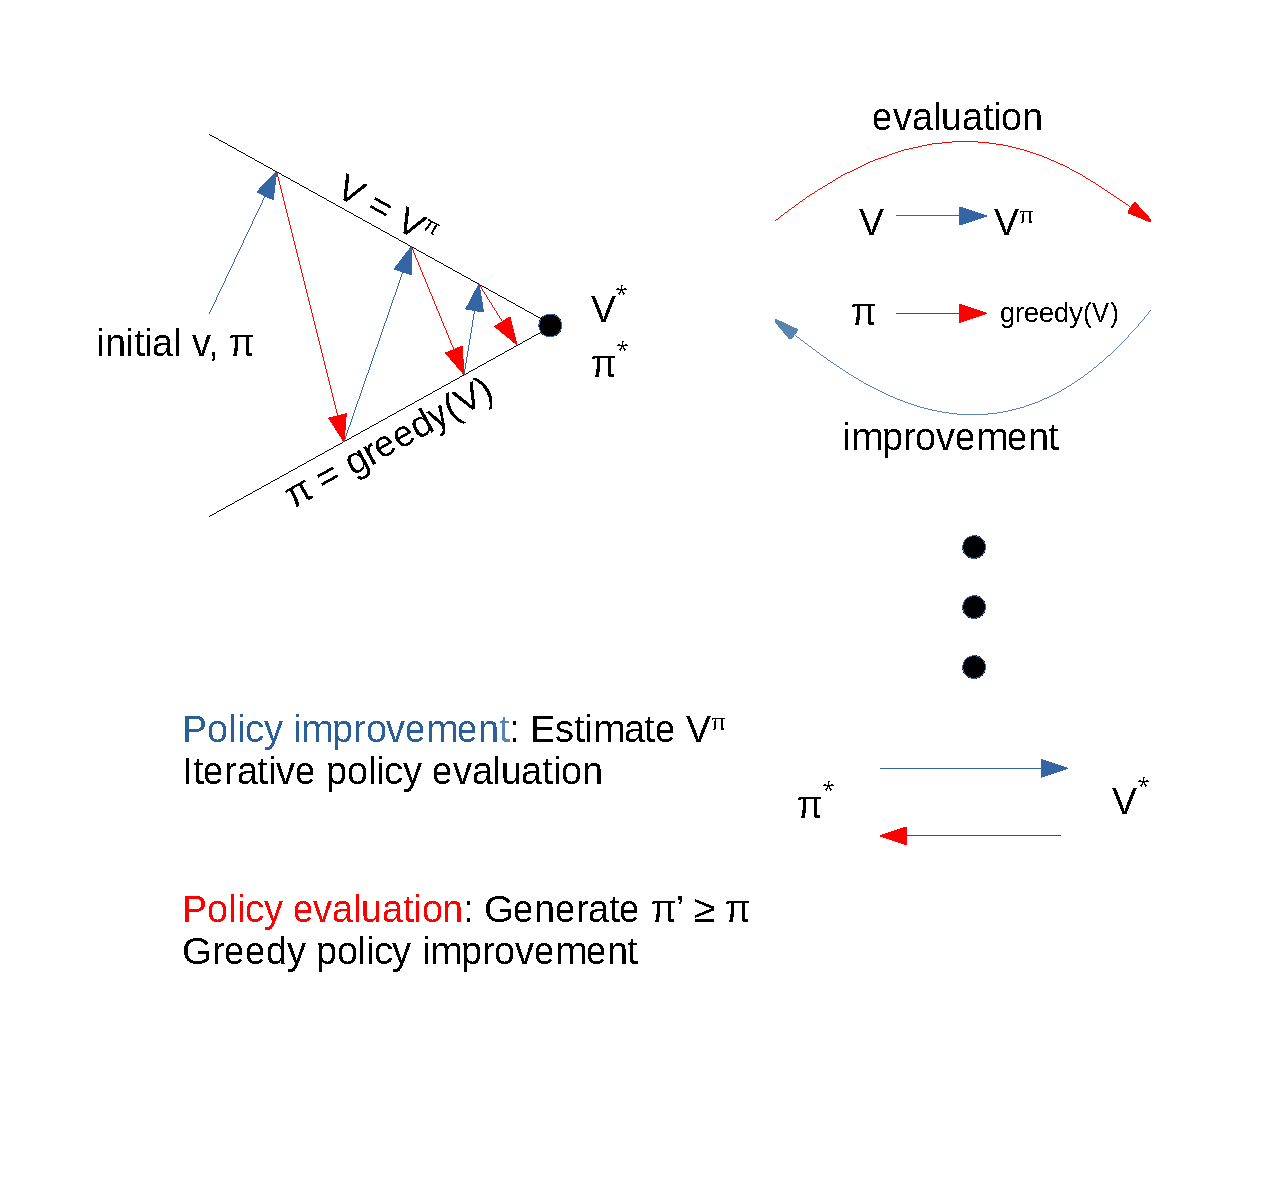
\includegraphics[width=1\linewidth]{MDP/fig/Policy_iteration.png}
		\caption{Greedy Policy iteration visualisation\cite{David_Silver}}
		\label{fig:greedy_policy_iteration}
	\end{subfigure}
	\caption{Policy Iteration \cite{David_Silver}}
	\label{fig:policy_iteration}
\end{figure}

\subsection{Policy Iteration}
There are two separate uses for Dynamic Programming in Reinforcement Learning. These are prediction and control which both have $(S,A,P,R,\gamma)$ as input.
\begin{itemize}
	\item The prediction method uses $(S,A,P,R,\gamma)$ and a policy $\pi$ as input, while it outputs a value function $v_\pi$.
	\item The control method only takes $(S,A,P,R,\gamma)$ as input and outputs the optimal value function $v_*$ and optimal policy $\pi_{*}$.
\end{itemize}
{\color{red} Maybe insert a flow diagram illustrating difference and similarity between prediction and control }

These two methods of Dynamic programming are implemented via what is known as value iteration and policy iteration respectively.
Figure \ref{fig:greedy_policy_iteration} shows how Greedy Policy Iteration works. A greedy policy is one which when followed, results in the maximum value function $v_\pi$. It is known that policy iteration converges which can also be seen in the diagram in Figure \ref{fig:greedy_policy_iteration} on the top left.\cite{sutton_barto}

As is stated in Figure \ref{fig:greedy_policy_iteration} policy iteration works by continuously iterating between two steps, namely policy evaluation and policy improvement.


For a given policy $\pi$ we improve the policy using the following two steps:\\\\
\textbf{Step one} is \textit{Evaluating} the policy $\pi$ using equation \ref{bellmanv2}: \[v_{\pi}(s) = E_{\pi}[R_{t+1} + \gamma v_{\pi}(S_{t+1})|S_t = s]\]
\textbf{Step two} is \textit{Improving} the policy by acting greedy with respect to $v_\pi$ to obtain a new policy $\pi^{'}$:
\begin{align}
	\pi^{'} &= greedy(v_{\pi})= v_{*}
	\label{pi'}
\end{align}
\[\pi^{'}(s) = \max\limits_{a}(R^{a}_s+\gamma\sum_{s'\in S}P^{a}_{ss'}v_*(s'))\]

What this means is that we obtain a value function by using iterative policy evaluation where after we update the policy. In this way we will always converge to the optimal policy $\pi_{*}$ and value function $v_{*}$ described by equation \ref{eq:pi_*} and \ref{bellmanv*} respectively.
\subsection{Value Iteration}
\begin{figure}[!htb]
	\centering
	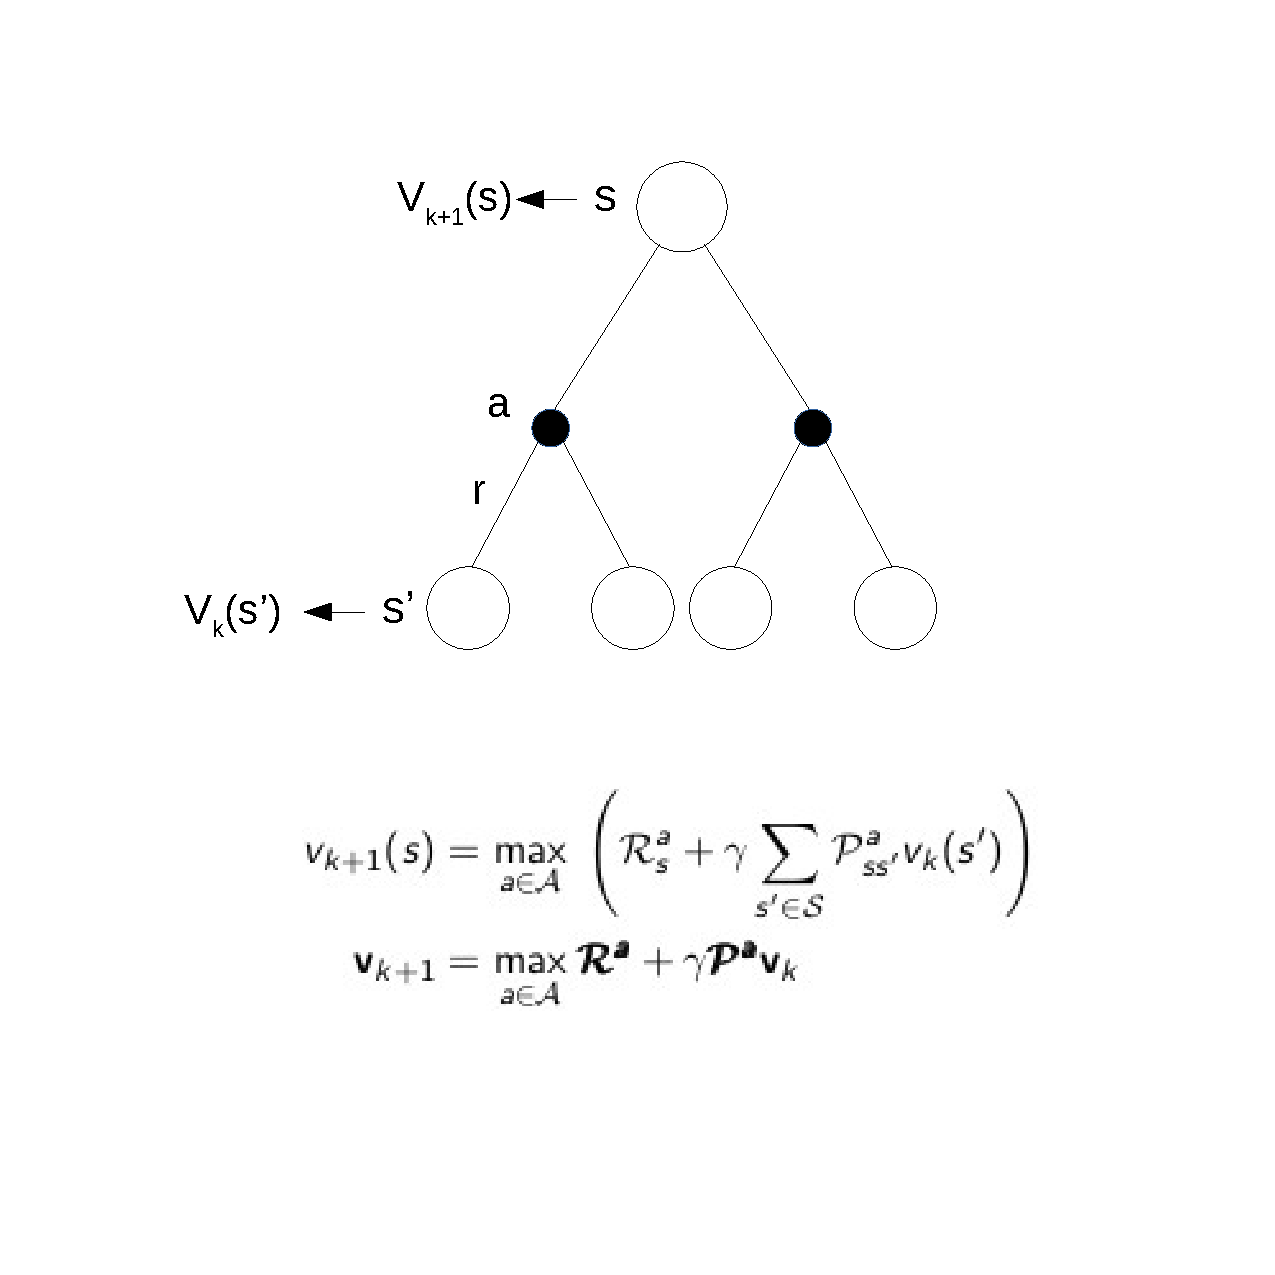
\includegraphics[width=0.75\linewidth]{MDP/fig/value_iteration.png}
	\caption{Value Iteration\cite{David_Silver}}
	\label{fig:value_iteration}
\end{figure}
Figure \ref{fig:value_iteration} shows the mathematics that describes \textit{Value Iteration}. It is very similar to iterative policy evaluation in Figure \ref{fig:iterative_policy_evaluation}. Iterative Policy Evaluation calculates the value function for a policy $\pi$ which is an entire set of actions given states.

While Value Iteration calculates the maximum value function for a single action only. In this sense Value Iteration is a special case of Iterative Policy Evaluation.

{\color{red} Can later place in appendix proof of policy iteration always converging. slide 19 (16/42) of David Silvers slides on Dynamic Programming}
\section{Reinforcement Learning}
What we have been discussing up to now all has had to do with using methods which required knowledge about the model. This knowledge was embedded in the probability transition matrix P. Often times this matrix P is extremely large making calculation times long. While at other times it is not possible to know the model of the environment beforehand. We therefore look at methods which do not need models.

There exists both model-free prediction and model-free control Reinforcement Learning techniques.
Model-free \textbf{prediction \textit{evaluates}} the value function of an unknown MDP.
While Model-free \textbf{control \textit{optimizes}} the value function of an unknown MDP.

There are two ways that model-free control can be implemented:

\textbf{On-policy learning:}
Learning characteristics of a policy $\pi$ by sampling from $\pi$

\textbf{Off-policy learning:}
Learn characteristics of policy $\pi$ by sampling another policy $\mu$

\subsection{Model-free prediction}
\subsubsection{Monte-Carlo Policy evaluation}
Monte-Carlo policy evaluation works as follows:
When time step t and state s is reached we increment a running counter N(s) = N(s)+1. This can be done in two ways, one being only incrementing N(s) the \textit{first} time state s is reached or incrementing N(s) \textit{every} time states s is reached.

Then we increment the total reward to S(s) =  S(s) + $G_t$.

Finally we calculate the value function $V(s)=\frac{S(s)}{N(s)}$

Then V(s) $\to V_\pi(s)$ as N(s) $\to \infty$

In order to incrementally do Monte-Carlo updates,an incremental mean $u_k$ is used. The derivation for $u_k$ from a standard mean is as follows:
\begin{align}
	u_k &= \frac{1}{k}\sum_{j=1}^{k}x_j\\
	&= \frac{1}{k}(x_k + \sum_{j=1}^{k-1}x_j)\\
	&= \frac{1}{k}(x_k +(k-1)u_{k-1})\\
	&= u_{k-1} + \frac{1}{k}(x_k - u_{k-1})
	\label{eq:u_k}
\end{align}
The variable that we are averaging over is V(s) hence $V(s)=u_{k-1}$ and the counter $N(s)=k$ in equation \ref{eq:u_k}. The return $G_t =x_k$. Hence at every time t:

\begin{align}
	N(S_t) &= N(S_t) + 1 \\
	V(S_t) &= V(S_t) + \frac{1}{N(S_t)}(G_t - V(S_t))
\end{align}
It can be useful to forget old states by making $N(S_t)$ a constant $\alpha$ as follows:
\[V(S_t) = V(S_t) + \alpha(G_t - V(S_t))\]

\subsubsection{Temporal Difference (TD) Learning}


\subsection{Model-free control}

When we previously used greedy policy improvement over the value function V(s) we had in equation \ref{pi'}:
\[\pi^{'}(s) = \max\limits_{a \in A}(R^{a}_s+\gamma\sum_{s'\in S}P^{a}_{ss'}v_*(s'))\]
Now for greedy policy improvement over the state action function Q(s,a) we have that:
\begin{equation}
	\pi^{'}(s) = \max\limits_{a \in A}Q(s,a)
\end{equation}
Which means that we now maximize not only across the action set as in equation \ref{pi'}, but rather the entire state-action set when using model-free policy iteration.

However there now arises a problem when always having the agent act greedily. Which is that the agent will always take the same path no matter whether another path might have been better in the long term. To overcome this limitation of we bring in the topic of $\epsilon$-Greedy exploration.

To ensure that the agent explores occasionally instead of always taking the greedy action, let the agent act randomly with a probability $\epsilon$. This can mathematically be expressed as:
\begin{align}
	\pi(a|s)=\begin{cases}
		\frac{\epsilon}{m}+1, & \text{if $a^* = \argmax\limits_{a \in A}Q (s,a)$}\\
		\frac{\epsilon}{m}, & \text{otherwise}
	\end{cases}
	\label{eq:pi_epsilon-greedy}
\end{align}
One can note that equation \ref{eq:pi_epsilon-greedy} is a variation of equation \ref{eq:pi_*}.


\graphicspath{{System\_Design/fig}}
\chapter{System Design}
\label{chap:System_Design}

\section{Introduction}
The 

To solve the puzzle I could have used monte carlo learning, ....
I chose SARSA and Q-learning because ...
\section{Thing 2}

\section{Methods}
\begin{itemize}
	\item Measure reward-episodes graphs
\end{itemize}
\graphicspath{{Experiments\_and\_Results/fig}}

\chapter{Applying reinforcement learning to sliding puzzles}
\label{chap:Experiments_and_Results}
\section{Introduction}
In the following section we will test the SARSA and Q-learning algorithms described in chapter \ref{chap:RL}. The way the tests will be conducted is by varying the hyper parameters. These hyper parameters include, the discount factor $\gamma$, epsilon the probability of choosing a random action and $\alpha$ the learning rate.

The puzzle that we will solve is of size 3x3. The way in which it will be solved is by training separate agents to solve different parts of the puzzle. 
\section{SARSA figs}

\section{Q-learning figs}

\section{Discussion}


\graphicspath{{conclusion/fig/}}

\chapter{Summary and Conclusion}
\label{chap:conclusion}

\section{Summary}
Objective 1 ...

Objective 2 ...

Objective 3 ...

So what? Relates back to problem and background sections in introductions.

\section{Future work and reccomendations}

% Bibliography
\bibliography{mybib}

% End matter
\appendix
\chapter{Project Planning Schedule}
\makeatletter\@mkboth{}{Appendix}\makeatother
\label{appen:derivations_bigramseg}

This is an appendix.

\chapter{Outcomes Compliance}
\makeatletter\@mkboth{}{Appendix}\makeatother
\label{appen:derivations_bigramseg}

This is another appendix.

\end{document}

